Onder dit kopje wordt er voornamelijk uitgelegd welke materialen en methoden er zijn gebruikt in het produceren van de Tetris gameboy. 
Daarnaast worden ook de deelvragen beantwoord die horen bij dit onderzoek. Ook wordt er uitgelegd hoe het spel vanuit de kant van de software en hardware precies werkt.  
\subsection{Systeem}
\label{subsec:methoden:systeem}
Een functioneel blokschema is een visuele representatie van een systeem of proces waarbij de componenten van het systeem op een abstract niveau worden weergegeven als blokken die verbonden zijn met lijnen. 
Het kan worden gebruikt om het ontwerp of de werking van een systeem te visualiseren, zoals in dit geval bij de Tetris gameboy \cite{earle1999engineering}. 

In dit project moest er ook een blokschema bedacht worden voor het Tetris spel. Deze blokschema bevat de volgende blokken en worden ook uitgelegd:
\begin{enumerate}
    \item Up, down, left en right: dit zijn de knopjes die nodig zijn om het spel te kunnen spelen. Elk knopje heeft zijn eigen functie, dit is dus het input systeem.
    \item Flash: de flash is nodig om de Tetris software op de PIC18F4520 te zetten. Dit is een bijzondere input om de microcontroller te kunnen programmeren.
    \item MCU (PIC18F4520): de microcontroller functioneert eigenlijk als het ``brein'' van het circuit. Deze microcontroller is verantwoordelijk voor het uitvoeren van de logica van het Tetris spel.
    \item IC (ULN2803A): deze IC is nodig om de LED matrixen te versterken en ook aan te sturen. Net als de MCU hoort dit tot de centrale verwerking van input en output.
    \item LED matrixen: deze zijn nodig om het beeld van spel te laten zien. Elk LEDje kan individueel aangestuurd worden, dit is dus het output systeem.
\end{enumerate}
De blokschema van het Tetris spel is te vinden in figuur \ref{fig:bdSimpel}.
\begin{figure}[h]
\centering
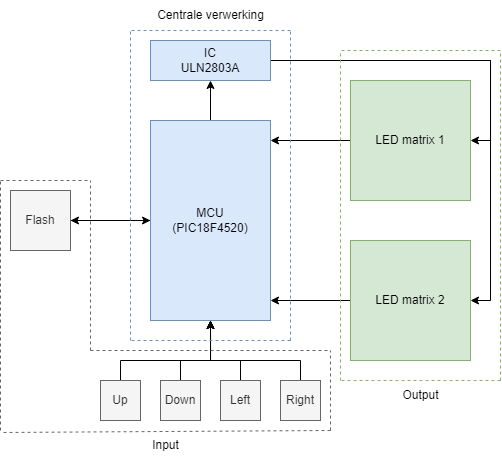
\includegraphics[width=0.85\columnwidth]{simpelBD.png}
\caption{Een blokschema ontwerp van het Tetris spelletje.}
\label{fig:bdSimpel}
\end{figure}

\subsection{Hardware}
\label{subsec:methoden:hardware}
Een licht emitterende diode (LED) is een half-geleidende component dat licht uitzendt met een klein kleurenspectrum wanneer stroom door de halfgeleider loopt. 
LED's kunnen licht uitstralen die overeenkomen met golflengten van ultraviolet tot infrarood licht.
Er bestaan verschillende soorten LED's, zoals de meest voorkomende LED soort: de traditionele 
``Through-hole'' LED. Je hebt ze in verschillende kleuren en maten. Deze ``Through Hole LED'' wordt meestal 
geleverd in 8mm, 5mm en 3mm qua grootte. Deze soort wordt meestal toegepast in simpele elektronische prototypen/apparaten en heeft als eigenschappen dat de LED minstens één kleur uitstraalt.

Naast deze traditionele through-hole LED zijn er ook vele andere soorten LED's.
Een aantal van deze LED soorten zal hieronder worden uitgewerkt:
\begin{enumerate}
    \item SMD (Surface Mounted Device) LED
    \item COB (Chip on Board) LED
    \item Bi-color LED
    \item Tri-color LED
    \item RGB-color LED
    \item Low-power LED
    \item High-power LED
    \item LED matrix: \ref{fig:LEDMATRIX}.
\end{enumerate}
\vspace{0.5cm}
\subsubsection{Surface Mounted Device LED}
Dit is een LED gemaakt voor printplaten met kleine elektronische circuits, zoals in smartphones of LED strips \cite{35285050LEDs}. Deze worden dan op de PCB 
gesoldeerd. Daarom heet dit component de "Surface Mounted Device", op z'n Nederlands 
noem je dit de ``Oppervlak Gemonteerde Component". De SMD LED wordt voornamelijk in computers en in PCB's gebruikt. Over 
de jaren heen zijn deze LEDjes steeds kleiner geworden, zodat er meer andere componenten 
op een PCB kunnen. In één SMB LED passen er meerdere LED's in.

Een van de eigenschappen van een SMD LED is dat ze zó minuscuul zijn, waardoor er weinig materiaal voor nodig is en bijna geen afval 
opleveren tijdens het productie proces. Daarnaast stralen deze LED's hoge intensiteit aan licht uit en werken ze ook op IC's \cite{LTSTS326KGKFKT}.
\\
\subsubsection{Chip on Board LED}
Een COB LED is ook een LED die op printplaten worden gesoldeerd. Het verschil 
tussen een COB LED en een SMB LED is dat de COB LED een grotere hoeveelheid licht uitstraalt 
ten opzichte van de SMB. Ook heeft de COB LED een optie om de lichtbundel te controleren.
De verhoudingen tussen het vermogen en lumen zijn veel beter dan die van de SMB LED, 
waardoor de productiviteit veel hoger is \cite{COBLEDs}. 

Meestal wordt een COB LED op een PCB toegepast in de computerwereld \cite{BSLCOB2503W030XXFR600320}.
\\
\subsubsection{Bi-color LED}
De bi-color LED is een LED die twee kleuren individueel kan uitstralen. 
Zoals de naam bi-color LED verklapt bevat deze LED soort twee kleuren LED's die parallel zijn geschakeld. De 
ene LED gaat aan als er een positieve lading staat op de kathode (negatieve pool) en de andere 
als er een positieve lading staat op de anode (positieve pool) \cite{TLUV5300}.

De belangrijke eigenschap van de bi-color LED is dat deze in staat is om twee verschillende kleuren kan uitstralen. 
Deze LED's hebben daarnaast ook als eigenschap een lange levensduur en een klein elektrische vermogen (zijn zuinig!) \cite{BiColorLED}.
\\
\subsubsection{Tri-color LED}
Een tri-color LED lijkt een beetje op de bi-color LED, maar is deze toch een beetje anders. 
De tri-color LED heeft drie poten, namelijk: groene en rode anode, en één ``common" kathode \cite{TriColourLED}. 
Deze tri-color LED wordt om die reden ook wel een bi-color LED genoemd met drie poten.
Als er een positieve lading staat op de groene anode, gaat er een groene licht branden. 
Als je alleen een positieve lading zet op de rode anode, gaat er een rode licht branden. 
Echter kun je ook positieve lading zetten op beide anodes, dat geeft een kleuren combinatie van groen en rood. 
Er zal dan een soort geel/ambergiek kleur uitgestraald worden. Daarnaast kun je ook met groen 
en rood ook andere kleuren maken door de PWM waarde aan te passen, 
dat wil zeggen dat je de spanningspercentage kunt instellen voor beide anodes. Daarmee kunnen andere kleurtinten worden gemaakt.  
In andere woorden: door de voltage te veranderen per LED kun je de helderheid aanpassen, 
waardoor je verschillende kleuren kunt maken. Dit is niet hetzelfde als bij een RGB LED, omdat je met een RGB LED wel alle kleuren kan maken met de drie primaire kleuren die je kunt beheren \cite{LD5911V2}.
\\
\subsubsection{Red-Green-Blue-color LED}
Een RGB-color LED is een LED die de drie primaire kleuren en combinatie van de primaire kleuren kan uitstralen, namelijk: 
rood, groen en blauw. Deze LED heeft dan ook vier poten: de common kathode, 
rode pin, groene pin en de blauwe pin. Net als dat je bij de tri-color LED bij de 
twee pinnen verschillende spanningen kunt voeden, kun je dat ook bij de RGB-color LED.
Je kunt dan verschillende spanningen toereiken aan elke van de drie pinnen, waardoor je alle 
mogelijke kleuren kunt creëren \cite{RGBLEDPinout}. Stel dat je de rode en blauwe poten maximale spanningsval geeft 
en dat je de groene poot de helft van die spanningsval toereikt, dan krijg je een paarse kleur 
met een extra effect!
\\
\subsubsection{Low-power LED}
Een low-power LED is een LED die weinig vermogen verbruikt zoals de naam dat ook verklapt. Deze LED's zijn 
extreem zuinig en kunnen ook in een compact uitvoering worden geleverd, maar hebben het nadeel dat ze  weinig licht opleveren. Low-power LED's werden gebruikt 
in de eerste LED lampen en tegenwoordig worden deze LED's gebruikt als indicator-lichting \cite{LEDPower}. 
Kortom zijn deze low-power LED's erg zuinig, compact, hebben een vermogen van 50 mW en geven helaas weinig licht \cite{EAPL2835RA0}.
\\
\subsubsection{High-power LED}
Een high-power LED verbruikt juist veel vermogen zoals de naam dat ook aangeeft. Deze LED's 
verbruiken minimaal 1 Watt aan vermogen \cite{FarnellDatasheet}. 
Naast dat ze veel vermogen nodig hebben geven deze LED's ook veel licht en hebben een grote lichtbundel. 
Nadeel is dat er rekening gehouden moet worden met de warmte productie van deze LED. 
Te veel warmte kan ervoor zorgen dat de levensduur van high-power LED sneller achteruit gaan en verouderen. 
Dat is ook de reden waarom er in sommige toepassingen van een high-power LED ook een koellichaam vereist wordt als deze continu gebruikt wordt \cite{LEDSupply}. 
In de datasheet wordt duidelijk aangegeven in welke toepassing en bij welke type LED een koellichaam vereist is. 
\\
\\
De elektrische eigenschappen van LED's kunnen variëren afhankelijk van de kleur van het licht dat ze produceren. 
Hieronder volgt een overzicht van de elektrische eigenschappen van de drie verschillende kleuren LED's:
\begin{table}[h]
    \centering    
    \caption{LED eigenschappen van de drie primaire kleuren.}
    \label{table:LEDs}
    \resizebox{\columnwidth}{!}{%
    \begin{tabular}{|l|l|l|l|l|l|}
    \hline
    \textbf{Kleur} & \textbf{Fabrikant} & \textbf{Half-geleider} & \textbf{Spanning (V)} & \textbf{Stroomsterkte (mA)} \\ \hline
    Rood  & Multicomp  \cite{redLED1} & AlGaAs & 2,0 & 20 \\ \hline
    Groen & Broadcom  \cite{greenLED1}  & InGaN & 3,2 & 20 \\ \hline
    Blauw & Kingbright \cite{blueLED1} & InGaN & 3,3 & 20 \\ \hline 
    \end{tabular}%
    }
    \end{table}

De waarden van elke LED van hun fabrikant die genoemd zijn in de tabel hierboven worden geverifieerd door de drie volgende andere fabrikanten:
\begin{enumerate}
    \item Rode LED: fabrikant 1 \cite{redLED1} wordt geverifieerd door fabrikant 2 \cite{redLED2}.
    \item Groene LED: fabrikant 1 \cite{greenLED1} wordt geverifieerd door fabrikant 2 \cite{greenLED2}.
    \item Blauwe LED: fabrikant 1 \cite{blueLED1} wordt geverifieerd door fabrikant 2 \cite{blueLED2}.
\end{enumerate}

\begin{figure}[h]
    \centering
    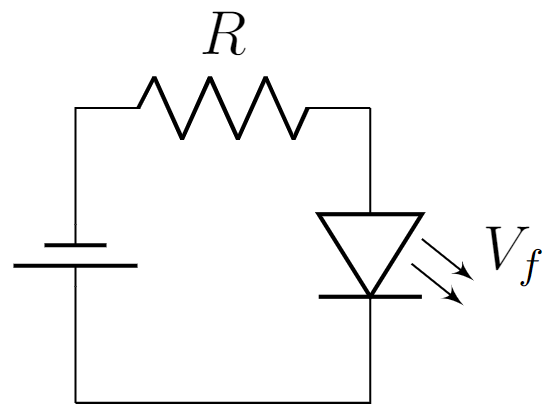
\includegraphics[width=0.3\columnwidth]{LEDcircuit.png}
    \caption{Een voorbeeld van een elektrisch circuit waarbij een LED en een weerstand in serie zijn geschakeld met een voedingsspanning (\(V_{bron}\)) van \(5V\).}
    \label{fig:LEDcircuit}
    \end{figure}

Als bijvoorbeeld de spanningsval van de LED \(2V\) is, en de voorwaartse stroomsterkte (\(I_f\)) \(20mA\) is, kan de stroomsterkte door de schakeling beter beperkt worden tot \(15mA\), zodat de LED minder snel beschadigd raakt. 
Om de waarde van de weerstand te bepalen, wordt de wet van Ohm toegepast \cite{Schagrin1963}:

\begin{center}\(I = \dfrac{(V_{bron} - V_f)}{R}\)\end{center}

Dan wordt de volgende berekening gebruikt om de waarde van de weerstand te bepalen:
\begin{enumerate}
    \item \(I = \frac{(5V - 2V)}{R}\)\\
    \item \(R = \frac{(5V - 2V)}{15mA}\)\\
    \item \(R = 180\Omega\)
\end{enumerate}
De weerstandswaarde van de weerstand moet gelijk zijn aan \(180\Omega\).
Als de stroom door de schakeling juist verhoogt moet worden kan er een kleinere weerstandswaarde gebruikt worden. 
Als de stroomsterkte juist verhoogt moet worden tot (\(20mA\)), wordt de volgende berekening gebruikt om de waarde van de weerstand te bepalen:
\begin{enumerate}
    \item \(I = \frac{(5V - 2V)}{R}\)\\
    \item \(R = \frac{(5V - 2V)}{20mA}\)\\
    \item \(R = 120\Omega\)
\end{enumerate}
De waarde van de weerstand moet gelijk zijn aan \(120\Omega\).
Aan de andere kant, als de stroom door de schakeling juist verlaagt moet worden, moet er een grotere weerstandswaarde worden gebruikt. 
Bijvoorbeeld als de stroom verlaagt moet worden tot 10 [mA], kan er met de volgende berekening de waarde van de weerstand bepaald worden:
\begin{enumerate}
    \item \(I = \frac{(5V - 2V)}{R}\)\\
    \item \(R = \frac{(5V - 2V)}{10mA}\)\\
    \item \(R = 300\Omega\)
\end{enumerate}
De waarde van de weerstand moet gelijk zijn aan \(300\Omega\).

Kortom is het belangrijk om een weerstandswaarde te kiezen die geschikt is voor de LED en de gewenste stroom, 
omdat een te hoge weerstandswaarde ertoe kan leiden dat de LED niet helder genoeg is. En bij een te lage weerstandswaarde kan dat ertoe leiden dat de LED beschadigd raakt of zelfs defect gaat \cite{ResistorForLED}. 

Een schakelaar aansluiten op een microcontroller (\(\mu C\)) vanuit een 5 V \(V_{cc}\) klinkt heel makkelijk, maar dat is het niet. 
De microcontroller moet namelijk een ``gedefinieerde toestand'' hebben, dat betekent simpel weg: aan of uit, binair gezien als 1 of 0. 
Als de schakelaar zoals de voorbeeld hierboven wordt aangesloten, zal de microcontroller geen gedefinieerde toestand hebben. 
Dit komt door een ``zwevende spanning'' \cite{saslow2007electricity}, dat is ruwweg vergelijkbaar met een ruis, zoals op een radio of een oude TV wanneer er geen zender beschikbaar is.
Ruis is eigenlijk een opname van willekeurig verschillende frequenties uitgezonden door andere apparaten. 
De draad die via de ingangspen naar de microcontroller gaat vangt die frequenties op via velden die niet gezien door het menselijk oog. 
Die frequenties zijn dan de ``zwevende spanningen'' en worden door de microcontroller afwisselend gezien als een 1 of 0, dus géén gedefinieerde toestand! 

Om dit probleem op te lossen worden er weerstanden gebruikt met een weerstandswaarde van meestal \(10k\Omega\). 
Deze weerstanden hebben een speciale naam, namelijk de ``pull-up'' of ``pull-down'' weerstand \cite{Platt2012-dz}. 
De schakelaar wordt tussen de aarde/massa (\(GND\)) en de ingangspen van de microcontroller geplaatst. 
Dit betekent dat de pull-up weerstand tussen de spanningsbron (\(V_{cc}\)) en de ingangspen van de microcontroller moet zitten.
Een pull-down weerstand wordt aangesloten tussen de ingangspen en de aarde, dus net andersom. 

Wanneer de schakelaar open staat wordt er een hoog signaal gelezen door de microcontroller, namelijk 5 V. 
Wordt de schakelaar ingedrukt, dan is het circuit gesloten en kan er zowel stroom naar de microcontroller als naar de grond lopen via de gesloten schakelaar. 
Op dat moment splitst de stroom en kan de microcontroller geen 5 V meer lezen en ziet de microcontroller dit als een laag signaal. 
Kortom: de ingangspen van de microcontroller wordt als het ware naar de hoge stand (pull-up) getrokken wanneer de schakelaar open staat. 
Je kunt daarnaast ook een pull-down weerstand gebruiken. Deze zorgt ervoor dat wanneer de schakelaar openstaat, dat er juist geen signaal gelezen kan worden, dus het signaal wordt naar beneden getrokken (pull-down) \cite{Platt2012-dz}.
In figuur \ref{fig:pullupexp} is het ontwerp van de pull-up weerstand schakelschema te zien en in figuur \ref{fig:pulldownexp} is het ontwerp van de pull-down weerstand schakelschema te zien.
\begin{figure}[h]
    \centering
    \begin{circuitikz}
        \draw (0,2) to [switch, mirror]  (0,0);  
        \draw (0,2) to  [R, l={$R_1$}, mirror] (0,5);
        \draw (0,2) -- (1,2);
        \draw (1,1) -- (1,3);
        \draw (1,1) -- (2,1);
        \draw (1,3) -- (2,3);
        \draw (2,1) -- (2,3);
        \draw (1.12,2) -- node[right] {$\mu C$} (1.12,2);
       \draw (0,0) node[ground]{};
       \draw (-0.3,5) --  node[anchor=south] {$+5V$} (0.3,5);
    \end{circuitikz}
    \caption{Een voorbeeldcircuit met een voedingsspanning, een pull-up weerstand, een ingangspen van een microcontroller, een drukknop en een massa (\(GND\)) \cite{circuitdigest_pullup_pulldown}.}
    \label{fig:pullupexp}
\end{figure}    
\begin{figure}[h]
    \centering
    \begin{circuitikz}
        \draw (0,2) to [switch, invert]  (0,5);  
        \draw (0,2) to  [R, l={$R_1$}, mirror] (0,0);
        \draw (0,2) -- (1,2);
        \draw (1,1) -- (1,3);
        \draw (1,1) -- (2,1);
        \draw (1,3) -- (2,3);
        \draw (2,1) -- (2,3);
        \draw (1.12,2) -- node[right] {$\mu C$} (1.12,2);
       \draw (0,0) node[ground]{};
       \draw (-0.3,5) --  node[anchor=south] {$+5V$} (0.3,5);
    \end{circuitikz}
    \caption{Een voorbeeldcircuit met een voedingsspanning, een drukknop, een ingangspen van een microcontroller, een pull-down weerstand en een massa (\(GND\)) \cite{circuitdigest_pullup_pulldown}.}
    \label{fig:pulldownexp}
\end{figure}\\

In dit project moest er ook gebruik gemaakt worden van een pull-down weerstand. In figuur \ref{fig:schakelcircuit} is de schakelschema van de Tetris gameboy te zien. 
In de schakelschema is het moeilijk te zien waar de pull-resistor precies zit. De common pin (COM) van de IC (ULN2803A) is verbonden met de voeding, dat is het kleine blokje dat in de afbeelding te zien is. 
Vanaf deze common pin gaat er een draad naar een $10k\Omega$ weerstand. Deze pull-up weerstand is dan weer doorverbonden naar de flash. 
De $10k\Omega$ pull-up weerstand zorgt ervoor dat de flash een gedefinieerde toestand heeft, wanneer deze niet in gebruik is. 
\begin{figure}[h]
    \centering
    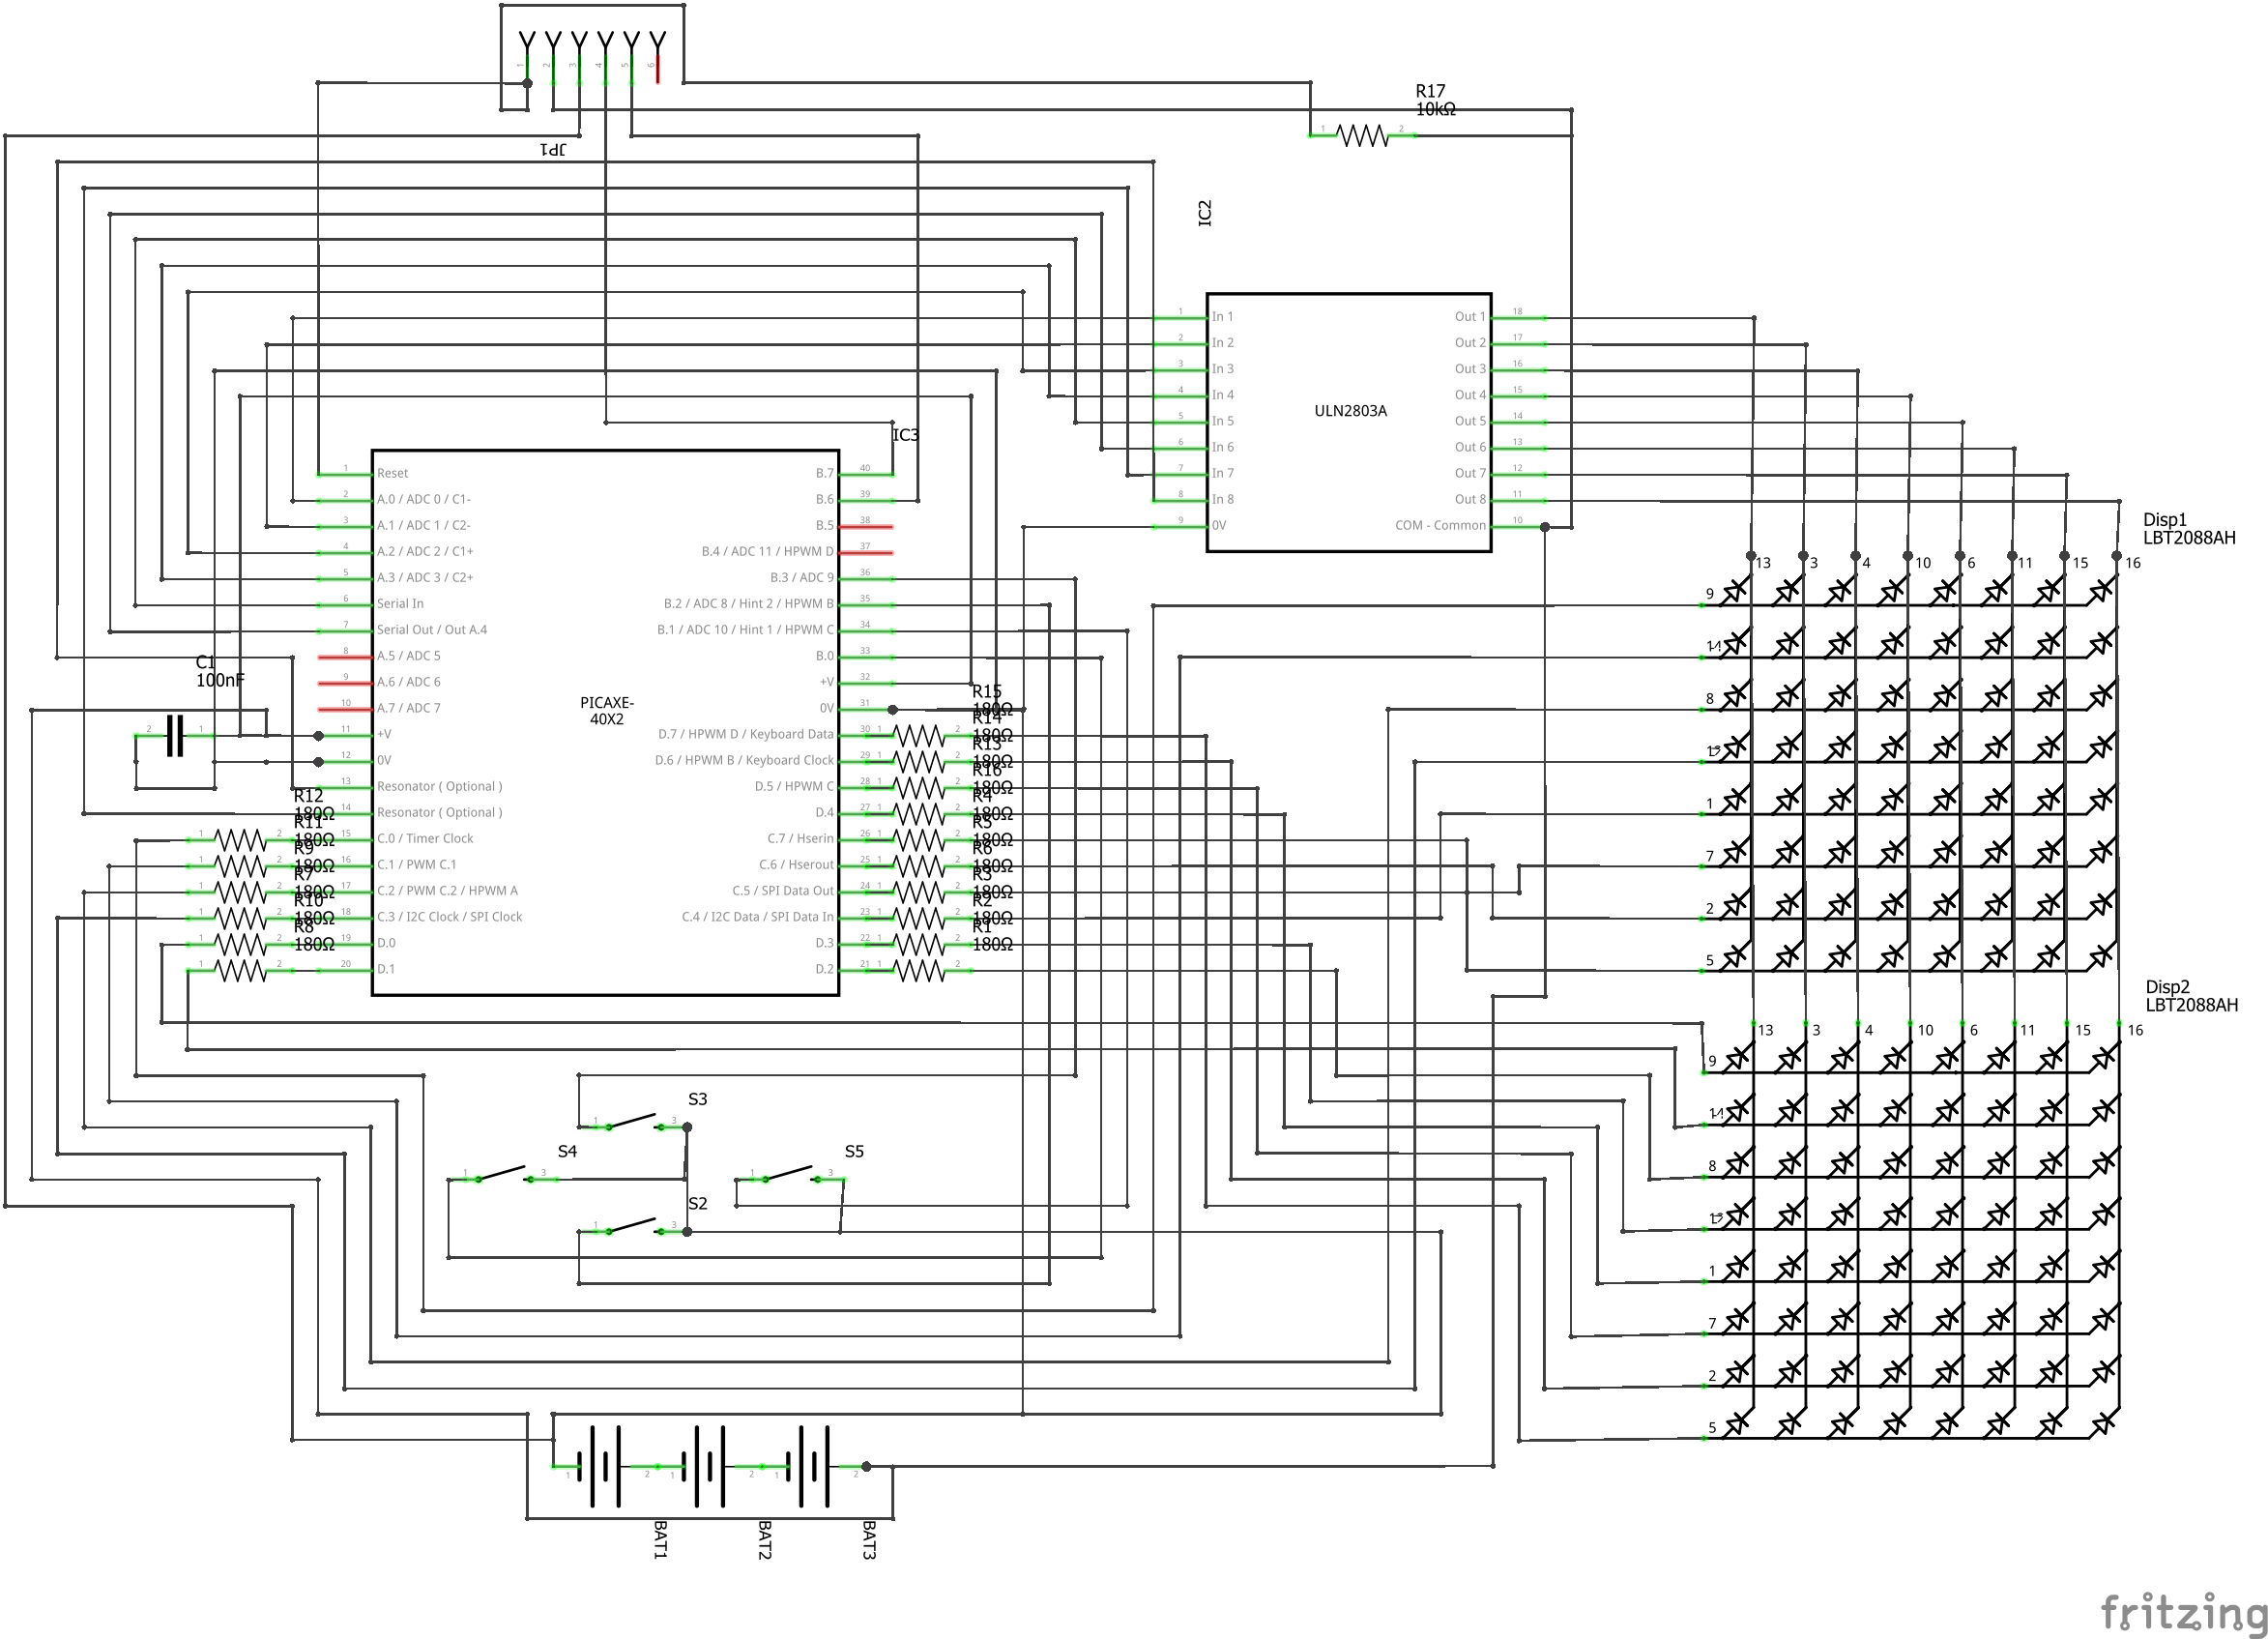
\includegraphics[width=1\columnwidth]{schakelschema.png}
    \caption{Zelf gemaakte schakelschema (in Fritzing) van de Tetris gameboy.}
    \label{fig:schakelcircuit}
    \end{figure}\\
Ook moest er gebruik gemaakt worden van twee 8x8 LED matrixen. Deze matrixen zorgen ervoor dat het spel wordt weergegeven voor de speler, dus dienen als output (userinterface). 
De LED matrix (ELM-2881SURWA/S530-A2) is een 8x8 array van rode LED's die op een bepaalde manier (matrix) met elkaar zijn aangesloten \cite{Everlight_ELM2881SURWA}. De LED's zijn allemaal individueel aanstuurbaar.  
In figuur \ref{fig:LEDMATRIX} is schema van de ELM-2881SURWA/S530-A2 LED matrix te zien. Het rechter schema van figuur \ref{fig:LEDMATRIX} is ook terug te zien in het schakelschema van het PICtris spel en is ook te zien hoe de twee matrixen zijn aangesloten: zie figuur \ref{fig:schakelcircuit}. 
De pinnen 9, 14, 8, 12, 1, 7 en 2 zijn gelimiteerd (met behulp van weerstanden) op een lagere stroomsterkte om de LED's niet te laten beschadigen. 
\begin{figure}[h]
    \centering
    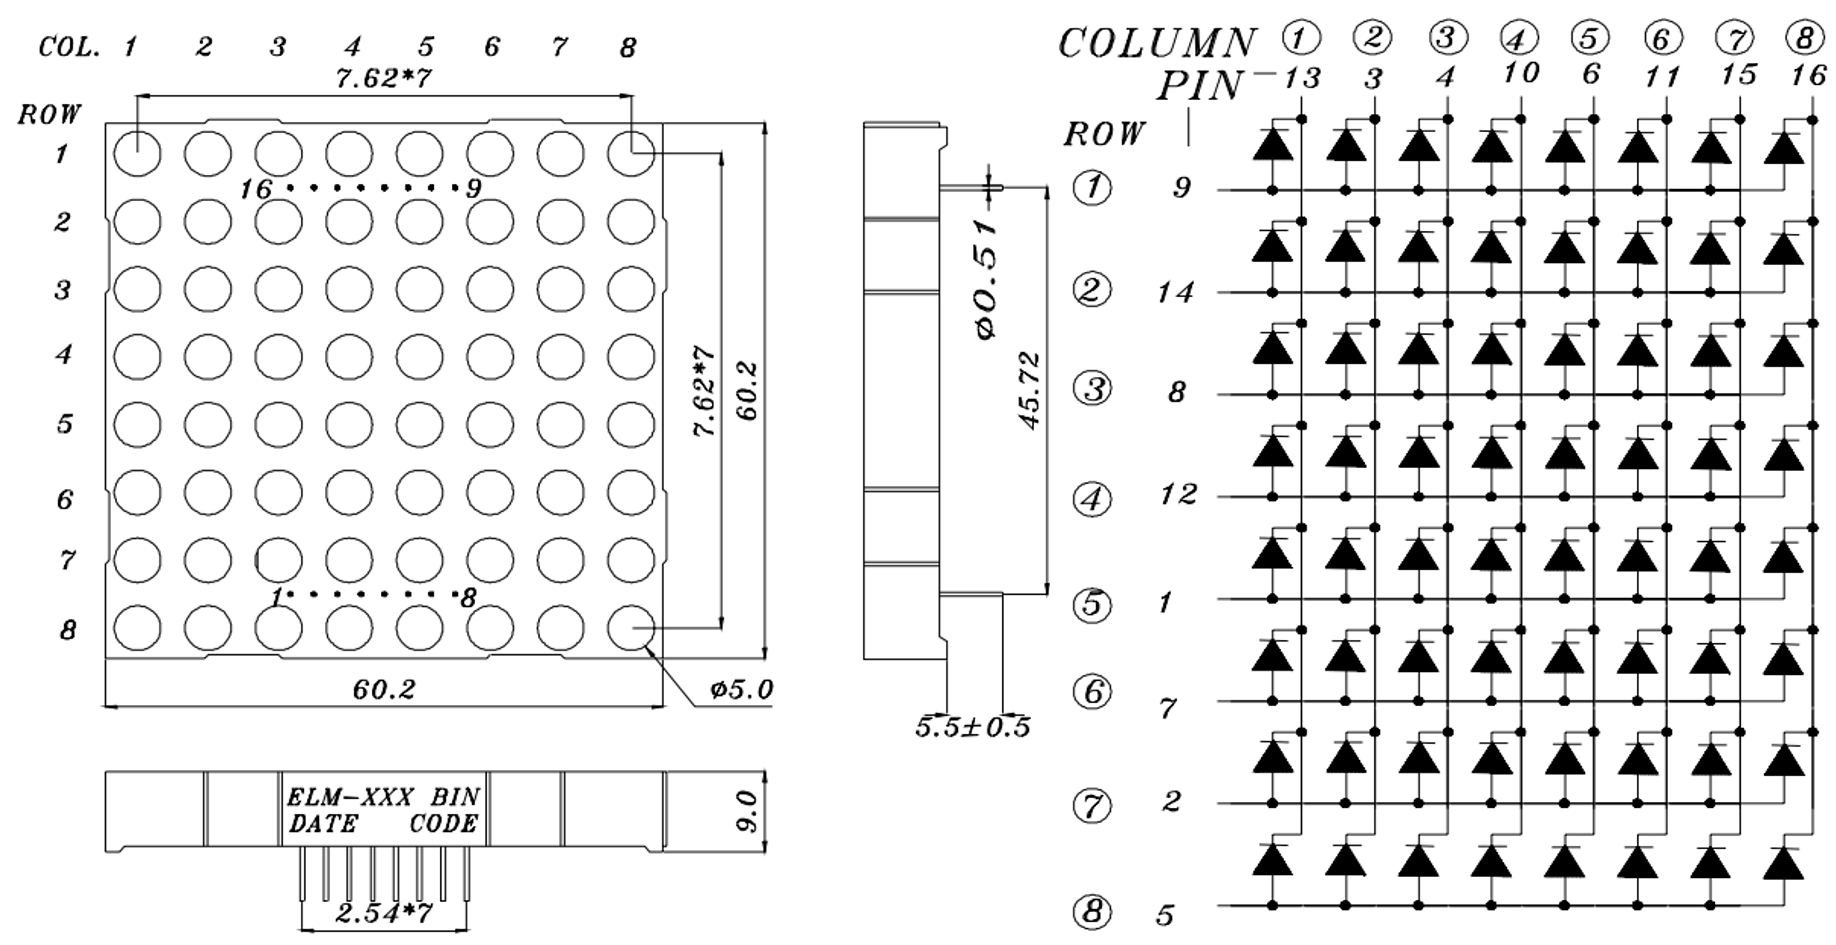
\includegraphics[width=0.85\columnwidth]{LEDMATRIX.png}
    \caption{Schema's van de ELM-2881SURWA/S530-A2 LED matrix \cite{Everlight_ELM2881SURWA}.}
    \label{fig:LEDMATRIX}
    \end{figure}\\

Tenslotte is er qua hardware nog gebruik gemaakt van een IC, namelijk de ULN2803A. 
De ULN2803A is een hoge spanning en hoge stroom Darlington transistor array \cite{ULN2803A_datasheet}, zie het rechter figuur in figuur \ref{fig:ULN}. Deze IC wordt meestal gebruikt om het digitale signaal van een ander component te versterken, omdat het component te weinig stroom levert. 
In het PICtris project is er hetzelfde probleem: de PIC18F4520 moet de LED matrixen aansturen met digitale signalen, maar de PIC18F4520 levert daarvoor te weinig stroom. 
Om dit probleem op te lossen is er in het circuit een extra IC (ULN2803A) toegevoegd die de zwakke digitale signalen van de PIC18F4520 versterkt, en daarna stuurt de ULN2803A het versterkte digitale signaal door naar de LED matrixen. 
In figuur \ref{fig:schakelcircuit} (schakelschema PICtris) is de ULN2803A terug te zien, daarbij is ook te zien hoe het digitale signaal wordt versterkt door een inkomende \(V_{dd}\) draad. Bovendien is deze common pin ook terug te zien in het linker deel van figuur \ref{fig:ULN}.
\begin{figure}[h]
    \centering
    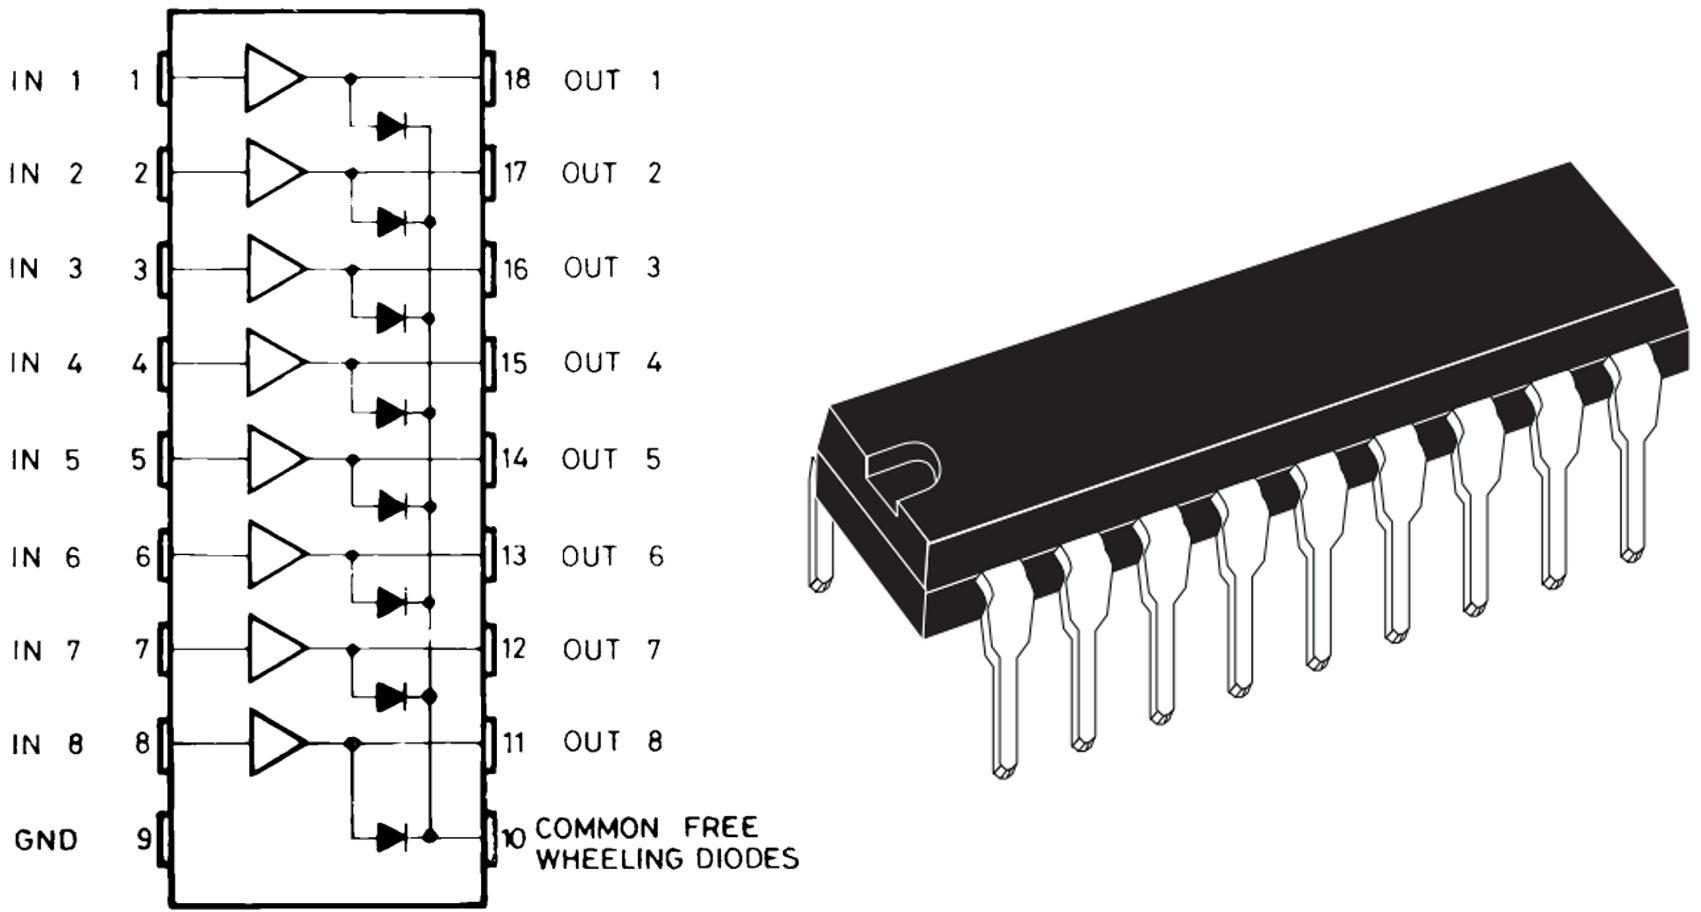
\includegraphics[width=0.85\columnwidth]{ULN.png}
    \caption{Schema's van de ULN2803A \cite{ULN2803A_datasheet}.}
    \label{fig:ULN}
    \end{figure}\\
In dit project was er een keuze mogelijk om de componenten van de Tetris gameboy te solderen op een protoboard/perfboard (geperforeerde bord) of op een zelf ontworpen PCB. 
Er is gekozen om de Tetris gameboy te realiseren op een perfboard. De reden daarvan is dat er meer flexibiliteit geeft en leerzamer is dan simpelweg de componenten op een ontworpen PCB te solderen. 
Een PCB is dan net iets mooier en beter qua design dan een perfboard. Bij een perfboard moet er uiteraard gebruik gemaakt worden van heel veel draadjes, wat bij een PCB juist niet hoeft. 
Er is gekozen om de perfboard design te maken in het softwareprogramma genaamd ``Fritzing'' \cite{Fritzing}, in figuur \ref{fig:perfPIC} wordt het ontwerp gerepresenteerd. 
Deze software is geschikt voor het designen van perfboard's. 
 
Er is gekozen om de ULN2803A IC horizontaal te plaatsen, omdat de output pinnen van de IC dan in dezelfde richting staan als die van de ELM2881SURWA LED matrixen. 
Het is dan makkelijker om de draden aan te sluiten en hoeven ze niet zoveel gebogen te worden. Daarnaast heeft de PIC18F4520 microcontroller nu genoeg ruimte om zich heen voor zijn eigen aansluitingen. 
De batterijhouder is linksonder geplaatst voor een betere grip voor het linker hand.
\begin{figure}[h]
    \centering
    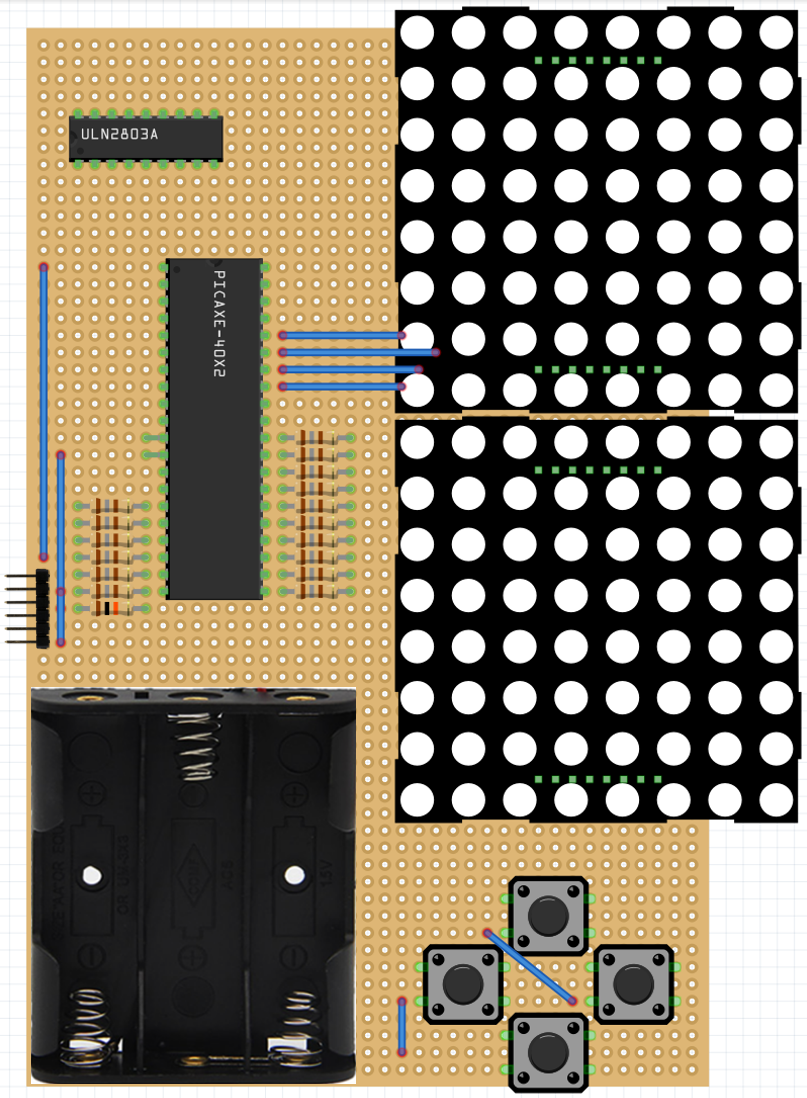
\includegraphics[width=0.612\columnwidth]{PROTOdesign.png}
    \caption{Perfboard Tetris gameboy design.}
    \label{fig:perfPIC}
    \end{figure}
\subsection{Software}
\label{subsec:methods:software}
% a short paragraph explaining/describing the software used in the system. no need to go deeply into the software. //
Het spel Tetris bestaat uit verschillende functies die de speler helpen het spel te spelen. 
Een van de belangrijkste functies is de mogelijkheid om de Tetromino's naar links of rechts te bewegen terwijl ze vallen, en ook de Tetromino's te kunnen draaien om ze in een betere oriëntatie te plaatsen.
Een andere belangrijke functie is de mogelijkheid om de valsnelheid van de Tetromino's te versnellen, waardoor de speler sneller lijnen kan wissen. 
Naast deze basis functies, zijn er nog paar andere functies die later behandeld zullen worden. 
Daarnaast zijn de spelregels al eerder uitgelegd in de introductie van dit artikel, deze is hier te vinden: \ref{sec:introduction}.

Deze functies zijn in combinatie met statements te schrijven als een algoritme. 
In dit project moest er een algoritme gemaakt worden, deze is te vinden in algoritme \ref{alg:tetris}. 
Hieronder zijn de functies die in het algoritme voorkomen nog uitgelegd:
\begin{enumerate}
    \item initialiseerMatrix(): initialiseert de twee 8x8 LED matrixen en zorgt ervoor dat alle LED's uitstaan.
    \item genereerTetromino(): genereert een nieuwe Tetromino aan de bovenkant van de LED matrix.
    \item verplaatsTetrominoNaarBeneden(): zorgt ervoor dat de Tetromino naar beneden valt met een bepaalde interval.
    \item draaiTetromino(): zorgt ervoor dat de Tetromino 90 graden naar rechts draait wanneer het knopje omhoog is ingedrukt.
    \item versnelTetrominoNaarBeneden(): zorgt ervoor dat de Tetromino versnelt naar beneden gaat wanneer het knopje omlaag is ingedrukt.
    \item checkLinksBewegingsMogelijkheid() en checkRechtsBewegingsMogelijkheid(): checken beide of er een collisie is tussen de vallende Tetromino en een andere Tetromino, of rand van de LED matrix. 
    \item verplaatsTetrominoNaarLinks(): als er geen collisie is, dan wordt de Tetromino naar links verplaatst met één vakje.
    \item verplaatsTetrominoNaarRechts(): als er geen collisie is, dan wordt de Tetromino naar rechts verplaatst met één vakje.
    \item checkCollisie(): checkt of de vallende Tetromino een collisie heeft met een andere Tetromino.
    \item controleerEnVerwijderVoltooideLijnen(): checkt of er voltooide lijnen zijn, en verwijderd de lijn(en) indien het nodig is.
    \item verhoogScore(): verhoogt de score wanneer er $x$ aantal rijen zijn verwijderd met $x$ aantal score.
\end{enumerate}
\renewcommand{\algorithmicrequire}{\textbf{Input:}}
\renewcommand{\algorithmicensure}{\textbf{Output:}}
\begin{algorithm}
    \caption{PICtris (Tetris) algorithm}
    \label{alg:tetris}
    \begin{algorithmic}[1]
    \REQUIRE Twee 8x8 LED matrixen, PIC18F4520, ULN2803A, een flash, Tetromino's, een score variable en de vier knopjes (speler input)
    \ENSURE Het spel PICtris wordt gespeeld op de twee 8x8 LED matrixen en de logica van het spel wordt uitgevoerd door de PIC18F4520.
    \STATE initialiseerMatrix()
    \WHILE{spelNietAfgelopen}
        \STATE genereerTetromino()
        \STATE verplaatsTetrominoNaarBeneden()
        \IF{omhoogKnop wordt ingedrukt}
            \STATE draaiTetromino()
        \ELSIF{naarBenedenKnop wordt ingedrukt}
            \STATE versnelTetrominoNaarBeneden()
        \ELSIF{linksKnop wordt ingedrukt}
            \IF{checkLinksBewegingsMogelijkheid()}
                \STATE verplaatsTetrominoNaarLinks()
            \ENDIF
        \ELSIF{rechtsKnop wordt ingedrukt}
            \IF{checkRechtsBewegingsMogelijkheid()}
                \STATE verplaatsTetrominoNaarRechts()
            \ENDIF
        \ENDIF
        \IF{checkCollisie()}
            \STATE vergrendelTetromino()
            \STATE controleerEnVerwijderVoltooideLijnen()
            \IF{$x$ aantal voltooide lijnen zijn verwijderd}
                \STATE verhoogScore()
            \ENDIF
        \ENDIF
        \IF{checkGameOver()}
            \STATE spelAfgelopen()
        \ENDIF
    \ENDWHILE
    \RETURN Score
    \end{algorithmic}
\end{algorithm}
\pagebreak